\documentclass{article}
\usepackage{CJKutf8}
\usepackage{amsmath}
\usepackage{amssymb}
\usepackage{amsfonts}
\usepackage{amsthm}
\usepackage{titlesec}
\usepackage{titletoc}
\usepackage{xCJKnumb}
\usepackage{tikz}


\usepackage{mathrsfs}

\newtheorem{Def}{定义}
\newtheorem{Thm}{定理}
\newtheorem{Exercise}{练习}

\newtheorem*{Example}{例}


\begin{document}
\begin{CJK*}{UTF8}{gbsn}
  \title{第一章 集合及其基本概念}
  \author{陈建文}
  \maketitle
  % \tableofcontents
  

% \underline{老师的话:}

% 我们首先要明确本门课程的两个学习目标。我们学习的过
% 程是围绕两个学习目标进行的,我们课程考试的内容也是按照我们的学习目标进
% 行设置的。

% 1)认真理解本课程中的每一个数学概念,对于学好本门课程是至关重要
% 的。这些数学概念将陪伴我们整个学习计算机科学的生涯。阅读并理解这些数学
% 概念的过程,对于培养我们将来描述计算机科学问题时准确的给出数学概念的能
% 力是非常重要的,这对应于我们抽象思维能力的培养。

% 2)认真理解本课程中的每一个证明过程,这对于培养我们的逻辑思维能力是至
% 关重要的。要想通过本课程的学习提升自己的逻辑思维能力,认真阅读并理解一
% 些重要定理的证明过程是必不可少的一个关键环节。如果我们只是记住一些定理,
% 没有理解定理的证明过程,要想取得一个好的考试成绩是很困难的。举例来说,
% 在中学时,我们学习了圆面积的计算公式$S=\pi
% r^2$,只需要掌握当$r=2$时,能够计算出$S=4\pi$即可。我们做了大量这样的习
% 题,最后能够取得一个好的考试成绩。但如果考试时要求我们证明$S=\pi r^2$,
% 如果我们没有理解该公式的证明过程,还能取得一个好的考试成绩吗?我们的期
% 末考试将以证明题为主,这与我们的学习目标是一致的。





  \begin{Def}
    通常把一些互不相同的东西放在一起所形成的整体叫做一个集合。构成集合的每个东西叫做集合的元素。
给定一个集合$A$和一个元素$a$,用$a \in A$表示$a$是$A$的一个元素,用$a \notin A$表示$a$不是$A$的一个元素。
  \end{Def}

  有两种方法表示一个集合:
\begin{enumerate}
\item 把构成集合的那些元素全部列出来
  \begin{itemize}
  \item $A = \{1, 2, 3\}$
\item $C = \{a, b, c, \ldots, z\}$
  \end{itemize}
\item 用概括集合中各元素的属性来表示集合$\{x|P(x)\}$
\begin{itemize}
\item $E = \{n|n \in \mathcal{Z} \land n\text{ is even}\}$,这里$\land$表示“并且”,$E$还可以等价的表示为$E = \{n \in \mathcal{Z} | n\text{ is even}\}$
\end{itemize}
\end{enumerate}

存在一个集合,该集合中不包含任何元素,称为空集,记为$\phi$。

  
\begin{Def}
设$A$,$B$为两个集合,如果$A$中的每个元素都是$B$中的元素,则称$A$为$B$的子集,记为$A \subseteq B$; 如果$A \subseteq B$且存在$x\in B$使得$x \notin A$,则称$A$为$B$的真子集,记为$A\subset B$。    
\end{Def}
\begin{itemize}
  \item   $\{1,2,4\} \subseteq \{1,2,3,4,5\}$
\item $\{1,2,4\} \subset \{1,2,3,4,5\}$
\end{itemize}

  $A\subseteq B: \forall x \in A x \in B$ 即$\forall x (x \in A \to x \in B)$
  
  $A\subset B: A \subseteq B \land \exists x\in B x \notin A$即$A \subseteq B \land \exists x (x\in B \land x \notin A)$

  设$A=\{1,2,4\},B=\{1,2,3,4,5\}$,则$A\subseteq B$,其含义是$\forall x x \in A \to x \in B$。
对一些特殊的$x$的值分析如下:
    \begin{itemize}
    \item 当$x = 1$时,$1 \in A \to 1 \in B$,即$T \to T$,其真值为$T$;
    \item 当$x = 3$时,$3 \in A \to 3 \in B$,即$F \to T$,其真值为$T$;
    \item 当$x = 0$时,$0 \in A \to 0 \in B$,即$F \to F$,其真值为$T$。
    \end{itemize}

  
    \begin{Def}
    设$A$,$B$为两个集合,如果$A \subseteq B$且$B \subseteq A$,则称$A$与$B$相等,并记为$A=B$。
  \end{Def}
    \begin{itemize}
  \item   $\{1,2,3,4,5\} = \{3,4,2,1,5\}$
\item $\{x \in \mathcal{R} | x^2 -5x + 6 = 0\} = \{2,3\}$
  \end{itemize}
  \begin{Thm}
   空集为任一个集合的子集且空集是唯一的。 
  \end{Thm}
  \begin{proof}[证明]
    设$A$为任意一个集合,显然对任意的$x$属于空集,则$x\in A$,因此空集为$A$的子集。

以下证明空集是唯一的。用反证法。假设存在两个不相等的空集$\phi$和$\phi'$,则$\phi \subseteq \phi'$并且$\phi' \subseteq \phi$,从而$\phi = \phi'$,矛盾。  
    
\end{proof}

“空集为任一集合的子集”这一结论初学时,也可以用反证法证明其正确性。

% 以帮助我们理解其中的逻辑。为了用反证法证明该结论,首先让我们分析一下对于任意的集合$A$和$B$,$A$不是$B$的子集($A\nsubseteq B$)的含义:
% \begin{equation*}
%   \begin{split}
%     A\nsubseteq B &\Leftrightarrow \lnot(A \subseteq B)\\
%     &\Leftrightarrow \lnot( \forall x x \in A \to x \in B)\\
%     &\Leftrightarrow \exists x \lnot(x \in A \to x \in B)\\
%     &\Leftrightarrow \exists x \lnot( \lnot (x \in A) \lor (x \in B))\\
%     &\Leftrightarrow \exists x (\lnot( \lnot (x \in A)) \land \lnot ( x \in B))\\
%     &\Leftrightarrow \exists x (x \in A \land x \notin B)\\
%   \end{split}
% \end{equation*}


   空集为任一个集合的子集。 
 \begin{proof}[证明]
   用反证法。设存在一个集合$A$,$\phi \nsubseteq A$,则存在$x\in \phi$,但$x \notin A$,这显然是不可能的,结论得证。   
 \end{proof}  
\begin{Def}
  集合$S$的所有子集构成的集合称为$S$的幂集,记为$2^S$或者$\mathcal{P}(S)$。
\end{Def}
\begin{Example}
      $2^{\phi}=\{\phi\}$

    $2^{\{1\}}=\{\phi, \{1\}\}$

  $2^{\{1,2\}}=\{\phi, \{1\},\{2\},\{1,2\}\}$
  
  $2^{\{1,2,3\}}=\{\phi, \{1\},\{2\},\{1,2\},\{3\},\{1,3\},\{2,3\},\{1,2,3\}\}$
\end{Example}

\begin{Example}
  $2^{\{\phi, \{\phi\}\}}=\{\phi, \{\phi\},\{\{\phi\}\}, \{\phi, \{\phi\}\}\}$
\end{Example}


{
\flushleft
\begin{minipage}{0.70\linewidth}
  \begin{Def}
    设$A,B$为任意的两个集合,至少属于集合$A$与集合$B$之一的那些元素构成的集合称为$A$与$B$的并集,记为$A \cup B$。
  \begin{equation*}
      A\cup B = \{x|x \in A \lor x \in B\} 
    \end{equation*}
    (这里$\lor$表示“或者”)
  \end{Def}
\end{minipage}
\begin{minipage}{0.29\linewidth}
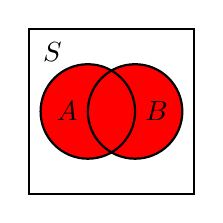
\begin{tikzpicture}[thick, scale=0.3]
  \draw (-3.5, -3.5) rectangle (3.5, 3.5);
  \filldraw[fill=red] (-1,0) circle [radius=2cm]
               (1,0) circle [radius=2cm];
  \draw (-1,0) node[left] {$A$};
  \draw (1,0) node[right] {$B$};
  \draw (-2.5,2.5) node {$S$};
\end{tikzpicture}
 \end{minipage}
}
\begin{Example}
  $\{1,2\} \cup \{2,3\} = \{1,2,3\}$
\end{Example}

{\flushleft
\begin{minipage}{0.70\linewidth}
  \begin{Def}
    设$A,B$为任意的两个集合,由既属于集合$A$又属于集合$B$的所有元素构成的集合称为$A$与$B$的交集,记为$A \cap B$。
    \begin{equation*}
      A\cap B = \{x|x \in A \land x \in B\}
    \end{equation*}
  \end{Def}
\end{minipage}
\begin{minipage}{0.29\linewidth}
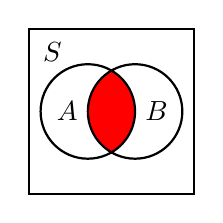
\begin{tikzpicture}[thick, scale=0.3]
  \draw (-3.5, -3.5) rectangle (3.5, 3.5);
  \fill[red] (-0.01, 0 |- -60:2cm) arc [start angle=-60, end angle = 60, radius = 2cm];
  \fill[red] (0.01, 0 |- 120:2cm) arc [start angle=120, end angle = 240, radius = 2cm];
  \draw (-1,0) circle [radius=2cm]
               (1,0) circle [radius=2cm];
  \draw (-1,0) node[left] {$A$};
  \draw (1,0) node[right] {$B$};
  \draw (-2.5,2.5) node {$S$};
\end{tikzpicture}
  \end{minipage}
    \begin{Example}
        $\{1,2\} \cap \{2,3\} = \{2\}$
    \end{Example}
  }

 {\flushleft
 \begin{minipage}{0.70\linewidth}
  \begin{Def}
    设$A,B$为任意的两个集合,由属于集合$A$但不属于集合$B$的所有元素构成的集合称为$A$与$B$的差集,记为$A \setminus B$。
    \begin{equation*}
      A\setminus B = \{x|x \in A \land x \notin B\}
    \end{equation*}
  \end{Def}
\end{minipage}
\begin{minipage}{0.29\linewidth}
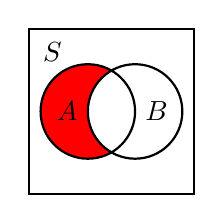
\begin{tikzpicture}[thick, scale=0.3]
  \draw (-3.5, -3.5) rectangle (3.5, 3.5);
\fill[red] (0,0 |- 60:2cm) arc [start angle=60, end angle = 300, radius = 2cm]
                           arc [start angle=240, end angle = 120, radius = 2cm];
  \draw (-1,0) circle [radius=2cm]
               (1,0) circle [radius=2cm];
  \draw (-1,0) node[left] {$A$};
  \draw (1,0) node[right] {$B$};
  \draw (-2.5,2.5) node {$S$};
\end{tikzpicture}
  \end{minipage}
    \begin{Example}
        $\{1,2\} \setminus \{2,3\} = \{1\}$
    \end{Example}
}

{\flushleft
\begin{minipage}{0.70\linewidth}
  \begin{Def}
    在许多实际问题中,常以某个集合$S$为出发点,而所涉及的集合都是$S$的子集。这个包含所考虑的所有集合的集合$S$,称为该问题的全集。如果$A$为$S$的子集,则差集$S \setminus A$称为集合$A$对集合$S$的补集,记为$A^c$。
    \begin{equation*}
      A^c = \{x|x \in S \land x \notin A\}
    \end{equation*}
  \end{Def}
\end{minipage}
\begin{minipage}{0.29\linewidth}
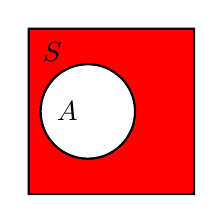
\begin{tikzpicture}[thick, scale=0.3]
  \filldraw[fill=red] (-3.5, -3.5) rectangle (3.5, 3.5)
               (-1, 0) circle [radius = 2cm];
  \draw (-1,0) node[left] {$A$};
  \draw (-2.5,2.5) node {$S$};
\end{tikzpicture}
\end{minipage}
}
    \begin{Example}
        $S = \{0,1\}, A =  \{0\},$ 则$A^c = \{1\}$。
    \end{Example}

\begin{Thm}
设$S$为全集,$\emptyset$为空集,$A$,$B$,$C$为$S$的子集,则\\
1. $A \cup B = B \cup A$, $A \cap B = B \cap A$.\\
2. $(A \cup B) \cup C = A \cup (B \cup C)$,$(A \cap B) \cap C = A \cap (B \cap C)$.\\
%3. $A \cup A = A$,$A \cap A = A$.\\
%4. $(A \cup B) \cap A = A$,$(A \cap B) \cup A = A$.\\
3. $A \cup \emptyset = A$, $A \cap \emptyset = \emptyset$.\\
4. $A \cup S = S$, $A \cap S = A$.\\
5. $A \cup (B \cap C) = (A \cup B) \cap (A \cup C)$, $A \cap (B \cup C) = (A \cap B) \cup (A \cap C)$.\\
6. $A \cup A^c = S$, $A \cap A^c = \emptyset$.\\
7. $C \setminus (A \cap B) = (C \setminus A) \cup (C \setminus B)$, $C\setminus (A \cup B) = (C \setminus A) \cap (C \setminus B)$.\\ 
7'.  $(A \cap B)^c = A^c \cup B^c$, $(A \cup B)^c = A^c \cap B^c$.\\
\end{Thm}
  以下只证明结论5和结论7的第一条,其他结论的证明留给读者自己完成。

  首先证明结论5的第一条,我们先在草稿纸上做如下的分析:
  \begin{equation*}
    \begin{split}
      \forall x &x \in A \cup (B \cap C)\\
      \Leftrightarrow& x \in A \lor x \in B \cap C\\
      \Leftrightarrow& x \in A \lor (x \in B \land x \in C)\\
      \Leftrightarrow& (x \in A \lor x \in B) \land (x \in A \lor x \in C)\\
      \Leftrightarrow& x \in A \cup B \land x \in A \cup C\\
      \Leftrightarrow& x \in (A \cup B) \cap (A \cup C)
    \end{split}
  \end{equation*}
  然后将上面的分析转化为证明如下:  
\begin{proof}[证明]
  先证$A \cup (B \cap C) \subseteq (A \cup B) \cap (A \cup C)$。

  对任意的$x$,如果$x \in A \cup (B \cap C)$,则 $x \in A$或者$x \in B \cap C$,从而$x \in A$,或者$x \in B$并且$ x \in C$,
  因此,$x \in A$或者$x \in B$,并且$x \in A$或者$ x \in C$,即,$x \in A \cup B$ 并且$x \in A \cup C$,于是,$x \in (A \cup B) \cap (A \cup C)$。

  再证$(A \cup B) \cap (A \cup C) \subseteq A \cup (B \cap C)$。

    对任意的$x$,如果$x \in (A \cup B) \cap (A \cup C)$,则 $x \in A \cup B$ 并且$x \in A \cup C$,从而$x \in A$或者$x \in B$,并且$x \in A$或者$ x \in C$,
  因此,$x \in A$,或者$x \in B$并且$ x \in C$,即,$x \in A$或者$x \in B \cap C$,于是,$x \in A \cup (B \cap C)$。

\end{proof}
接下来证明结论7的第一条,我们先在草稿纸上做如下的分析:
\begin{equation*}
  \begin{split}
    \forall x &x \in C\setminus (A\cap B)\\
    \Leftrightarrow&x \in C \land x \notin A\cap B\\
    \Leftrightarrow&x \in C \land \lnot (x \in A\cap B)\\
    \Leftrightarrow&x \in C \land \lnot (x \in A \land x \in B)\\
    \Leftrightarrow&x \in C \land (\lnot (x \in A) \lor \lnot (x \in B))\\
    \Leftrightarrow&x \in C \land (x \notin A \lor x \notin B)\\
    \Leftrightarrow&(x \in C \land x \notin A) \lor (x \in C \land x \notin B)\\
    \Leftrightarrow&(x \in C\setminus A)\lor (x\in C\setminus B)\\
    \Leftrightarrow&x \in (C\setminus A) \cup (C \setminus B)
  \end{split}
\end{equation*}
然后将上面的分析转化为证明如下:  
\begin{proof}[证明]
  先证$C\setminus (A\cap B)\subseteq (C\setminus A) \cup (C \setminus B)$。

  对任意的$x$,如果$x \in C\setminus (A\cap B)$,则$x \in C$并且$x \notin A\cap B$,从而$x \in C$并且$x\notin A$或者$x\notin B$,因此,$x\in C\setminus A$或者$x\in C\setminus B$,于是$x\in (C\setminus A) \cup (C \setminus B)$。

  再证$(C\setminus A) \cup (C \setminus B) \subseteq C\setminus (A\cap B)$。

  对任意的$x$,如果$x\in (C\setminus A) \cup (C \setminus B)$, 则$x\in C\setminus A$或者$x\in C\setminus B$,从而$x \in C$并且$x\notin A$或者$x\notin B$,因此,$x \in C$并且$x \notin A\cap B$,于是$x \in C\setminus (A\cap B)$。
\end{proof}
\begin{Example}
下列等式是否成立?

  $(A\setminus B)\cup C = A\setminus (B\setminus C)$

  若成立,请给出证明。若不成立,请说明理由。

  
\end{Example}
\begin{proof}[答]
  该等式不成立。设$A=\phi$, $B=\phi$,$C=\{0\}$,则$(A\setminus B)\cup C= \{0\}$,而$A\setminus (B\setminus C)=\phi$,  $(A\setminus B)\cup C \neq A\setminus (B\setminus C)$。
\end{proof}
{\flushleft
\begin{minipage}{0.69\linewidth}
  \begin{Def}
    设$A,B$为任意的两个集合,$A\setminus B$与$B\setminus A$的并集称为$A$与$B$的{\bfseries 对称差},记为$A \bigtriangleup B$。
    \begin{equation*}
      A\bigtriangleup B = (A \setminus B) \cup (B \setminus A)
    \end{equation*}
  \end{Def}
\end{minipage}
\begin{minipage}{0.29\linewidth}
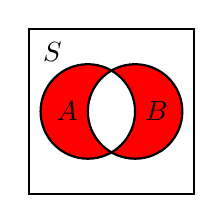
\begin{tikzpicture}[thick, scale=0.3]
  \draw (-3.5, -3.5) rectangle (3.5, 3.5);
\fill[red] (0,0 |- 60:2cm) arc [start angle=60, end angle = 300, radius = 2cm]
                           arc [start angle=240, end angle = 120, radius = 2cm];
\fill[red] (0,0 |- 60:2cm) arc [start angle=120, end angle = -120, radius = 2cm]
                           arc [start angle=-60, end angle = 60, radius = 2cm];
  \draw (-1,0) circle [radius=2cm]
               (1,0) circle [radius=2cm];
  \draw (-1,0) node[left] {$A$};
  \draw (1,0) node[right] {$B$};
  \draw (-2.5,2.5) node {$S$};
\end{tikzpicture}
  \end{minipage}}
\begin{Example}
  \begin{align*}
      &\{1,2\} \bigtriangleup \{2,3\} = \{1,3\}\\
      &\{1,2\} \bigtriangleup \{1\} = \{2\}\\
      &\{1,2\} \bigtriangleup \phi = \{1,2\}\\
      &\{1,2\} \bigtriangleup \{1,2\}=\phi    
  \end{align*}
      \end{Example}

      \begin{Thm}
        设$A,B$为任意两个集合,则
        \begin{equation*}
          A \bigtriangleup B = (A \cap B^c)\cup (A^c \cap B)
        \end{equation*}
      \end{Thm}
  \begin{Thm}
设$A,B,C$为任意三个集合,则\\
1. $A \bigtriangleup B = B \bigtriangleup A$.\\
2. $(A \bigtriangleup B) \bigtriangleup C = A \bigtriangleup (B \bigtriangleup C)$.\\
3. $\emptyset \bigtriangleup A = A$.\\
4. $A \bigtriangleup A = \emptyset$.\\
5. $A \cap (B \bigtriangleup C) = (A \cap B) \bigtriangleup (A \cap C)$.\\ 
  \end{Thm}

 以下证明结论2和结论5,其他结论留给读者思考。 先证明结论2。

\begin{proof}[证明]

  
  因为
  \begin{equation}
  x \in A \bigtriangleup B \Leftrightarrow
  (x \in A \land x \notin B) \lor (x \notin A \land x
  \in B),    
  \end{equation}

  所以
  \begin{equation}
    \begin{split}
      x \notin A \bigtriangleup B &\Leftrightarrow \lnot (x\in A \bigtriangleup B)\\
      &\Leftrightarrow \lnot((x \in A \land x \notin B) \lor (x \notin A \land x
      \in B))\\
      &\Leftrightarrow \lnot(x \in A \land x \notin B) \land \lnot(x \notin A \land x
      \in B)\\
      &\Leftrightarrow
  (x \notin A \lor x \in B) \land (x \in A \lor x
  \notin B)\\
  &\Leftrightarrow
  ((x \notin A \lor x \in B) \land x \in A) \lor
  ((x \notin A \lor x \in B) \land  x
  \notin B)\\
  &\Leftrightarrow
  ((x \notin A \land x \in A)\lor (x \in B \land  x \in A) ) \\
  &\lor
  ((x \notin A \land  x
  \notin B) \lor (x \in B \land  x
  \notin B) )\\
  &\Leftrightarrow  (x \in A \land x \in B ) \lor(x \notin A \land x \notin B) 
    \end{split}
  \end{equation}

  于是
  \begin{equation}\label{xor1}
    \begin{split}
      &x \in (A \bigtriangleup B) \bigtriangleup C\\
      &\Leftrightarrow (x \in A \bigtriangleup B \land x \notin C) \lor (x \notin A \bigtriangleup B \land x \in C)\\
      &\Leftrightarrow (((x \in A \land x \notin B) \lor (x \notin A \land x \in B)) \land x \notin C)\\
      &\lor (((x \in A \land x \in B ) \lor(x \notin A \land x \notin B)) \land x \in C)\\
      &\Leftrightarrow (x \in A \land x \notin B \land x \notin C) \lor (x \notin A \land x \in B \land x \notin C)\\
      &\lor (x \notin A \land x \notin B \land x \in C) \lor (x \in A \land x \in B \land x \in C)
    \end{split}
  \end{equation}

  \begin{equation}\label{xor2}
    \begin{split}
      &x \in A \bigtriangleup (B \bigtriangleup C)\\
      &\Leftrightarrow x \in (B \bigtriangleup C) \bigtriangleup A\\
      &\Leftrightarrow (x \in A \land x \notin B \land x \notin C) \lor (x \notin A \land x \in B \land x \notin C)\\
      &\lor (x \notin A \land x \notin B \land x \in C) \lor (x \in A \land x \in B \land x \in C)
    \end{split}
  \end{equation}
  其中\eqref{xor2}式的第二行由对称差运算的交换律得到,\eqref{xor2}式的第三行由与
   \eqref{xor1}式的对称性得到。

  由\eqref{xor1}式和\eqref{xor2}式可得
  $(A\bigtriangleup B)\bigtriangleup C = A\bigtriangleup (B\bigtriangleup C)$。
\end{proof}

再证明结论5。

\begin{proof}[证明]
   \begin{align}
    &A\cap (B\bigtriangleup C)\nonumber \\
    =&A\cap (B\setminus C \cup C\setminus B) \nonumber \\
    =&(A\cap B\setminus C) \cup (A \cap C\setminus B) \label{eq:first} \\      
    &(A\cap B)\bigtriangleup (A\cap C) \nonumber \\
    =&(A\cap B)\setminus (A\cap C) \cup (A\cap C)\setminus (A\cap B) \nonumber \\
    =&(A\cap B)\setminus A \cup (A\cap B)\setminus C \cup (A\cap C)\setminus A \cup (A\cap C)\setminus B \nonumber \\
    =&(A\cap B)\setminus C \cup (A\cap C)\setminus B \nonumber \\
    =&(A\cap B\setminus C) \cup (A \cap C\setminus B)\label{eq:second}      
   \end{align}
由式\eqref{eq:first}和式\eqref{eq:second}知$A\cap (B\bigtriangleup C)=(A\cap B)\bigtriangleup (A\cap C)$。
\end{proof}
  \begin{Def}  
    以集合为元素的集合称为集族。如果$I$为任意一个集合,对$I$中每个元素$\alpha$都有一个唯一的集合与之对应,这个集合记为$A_{\alpha}$,那么所有这些$A_{\alpha}$形成的集族可以用$\{A_{\alpha}\}_{\alpha \in I}$表示,其中$I$称为标号集。
  \end{Def}
  \begin{Def}
    集族$\{A_{\alpha}\}_{\alpha \in I}$中所有集合的并集$\bigcup_{\alpha \in I}A_{\alpha}$定义为
\[ \bigcup_{\alpha \in I}A_{\alpha} = \{x|\exists \alpha \in I  x \in A_{\alpha}\}\]
    集族$\{A_{\alpha}\}_{\alpha \in I}$中所有集合的交集$\bigcap_{\alpha \in I}A_{\alpha}$定义为
\[ \bigcap_{\alpha \in I}A_{\alpha} = \{x|\forall \alpha \in I x \in A_{\alpha}\}\]
  \end{Def}
\begin{Example}
  如果$I=\{1,2,3\}$,则$\bigcup_{\alpha \in I}A_{\alpha} =A_1\cup A_2\cup A_3$;

    如果$I=\{1,2,3\}$,则$\bigcap_{\alpha \in I}A_{\alpha} =A_1\cap A_2\cap A_3$;

    如果$I=\mathbb{N}$,则$\bigcup_{\alpha \in I}A_{\alpha} =A_0\cup A_1\cup A_2\cup\cdots=\bigcup_{\alpha=0}^{\infty}A_{\alpha}$;
    
    如果$I=\mathbb{N}$,则$\bigcap_{\alpha \in I}A_{\alpha} =A_0\cap A_1\cap A_2\cap\cdots=\bigcap_{\alpha=0}^{\infty}A_{\alpha}$;

    如果$I=\mathbb{Z}^+$,则$\bigcup_{\alpha \in I}A_{\alpha} =A_1\cup A_2\cup A_3\cup\cdots=\bigcup_{\alpha=1}^{\infty}A_{\alpha}$;
    
    如果$I=\mathbb{Z}^+$,则$\bigcap_{\alpha \in I}A_{\alpha} =A_1\cap A_2\cap A_3\cap\cdots=\bigcap_{\alpha=1}^{\infty}A_{\alpha}$。
\end{Example}
  \begin{Example}
    设$I=\{x \in \mathbb{R} | 0 < x \leq 1\}$,$\forall x \in \mathbb{R}, A_x=\{y\in \mathbb{R}|0 < y < x\}$,
    则
    \begin{equation*}
      \bigcup_{x\in I}A_x=\{x \in \mathbb{R} | 0 < x < 1\},
      \bigcap_{x\in I}A_x=\phi      
    \end{equation*}
  \end{Example}

  \begin{Thm}
设$A$为任意集合, $\{B_{\alpha}\}_{\alpha \in I}$为任意一个集族,则
\begin{enumerate}
  \item $A \cup (\bigcap_{\alpha \in I}B_{\alpha}) = \bigcap_{\alpha \in I}(A \cup B_{\alpha})$
  \item $A \cap (\bigcup_{\alpha \in I}B_{\alpha}) = \bigcup_{\alpha \in I}(A \cap B_{\alpha})$
\end{enumerate}
\end{Thm}
\begin{proof}[证明]
  留给读者自己完成。
\end{proof}
\begin{Thm}
  设$C$为任意集合, $\{A_{\alpha}\}_{\alpha \in I}$为任意一个集族,则
  \begin{enumerate}
  \item $C\setminus(\bigcap_{\alpha \in I}A_{\alpha})=\bigcup_{\alpha\in I}(C\setminus A_{\alpha})$
  \item $C\setminus(\bigcup_{\alpha \in I}A_{\alpha})=\bigcap_{\alpha\in I}(C\setminus A_{\alpha})$
  \end{enumerate}
  \end{Thm}
  以下只证明第1条,其他结论的证明留给读者自己完成。

  我们先在草稿纸上做如下的分析:

  \begin{equation*}
    \begin{split}
      \forall x&x \in C\setminus (\bigcap_{\alpha \in I}A_{\alpha})\\
      \Leftrightarrow &x \in C \land x \notin \bigcap_{\alpha \in I}A_{\alpha}\\
      \Leftrightarrow &x \in C \land \lnot (x \in \bigcap_{\alpha \in I}A_{\alpha})\\
      \Leftrightarrow &x \in C \land \lnot (\forall \alpha \alpha \in I \to x \in A_{\alpha})\\
      \Leftrightarrow &x \in C \land \exists \alpha \lnot (\alpha \in I \to x \in A_{\alpha})\\
      \Leftrightarrow &x \in C \land \exists \alpha \lnot (\lnot (\alpha \in I) \lor x \in A_{\alpha})\\
      \Leftrightarrow &x \in C \land \exists \alpha \lnot \lnot (\alpha \in I) \land \lnot x\in A_{\alpha}\\
      \Leftrightarrow &x \in C \land \exists \alpha (\alpha \in I \land x\notin A_{\alpha})\\
      \Leftrightarrow &\exists \alpha (\alpha \in I \land x\in C \land x \notin A_{\alpha})\\
      \Leftrightarrow &\exists \alpha (\alpha \in I \land x\in C\setminus A_{\alpha})\\
      \Leftrightarrow &x \in \bigcup_{\alpha \in I} (C\setminus A_{\alpha}) \\
    \end{split}
  \end{equation*}
  然后将上面的分析转化为证明如下:  
  \begin{proof}[证明]
    先证明$C\setminus(\bigcap_{\alpha \in I}A_{\alpha})\subseteq \bigcup_{\alpha\in I}(C\setminus A_{\alpha})$。

  对任意的$x$,如果$x \in C\setminus (\bigcap_{\alpha \in I}A_{\alpha})$,则$x\in C$,且$x \notin \bigcap_{\alpha \in I}A_{\alpha}$,从而$x\in C$,且存在$\alpha \in I$,$x\notin A_{\alpha}$。于是,存在$\alpha \in I$,$x\in C\setminus A_{\alpha}$。因此,$x \in \bigcup_{\alpha \in I}( C\setminus A_{\alpha})$,故$C\setminus (\bigcap_{\alpha \in I}A_{\alpha})\subseteq \bigcup_{\alpha\in I}(C\setminus A_{\alpha})$。

    其次,对任意的$x$,如果$x\in \bigcup_{\alpha\in I}(C\setminus A_{\alpha})$,则存在$\alpha \in I$,$x\in C\setminus A_{\alpha}$。因此,存在$\alpha \in I$,$x\in C$且$x\notin A_{\alpha}$,故$x\in C$且$x\notin \bigcap_{\alpha \in I}A_{\alpha}$。于是,$x \in C\setminus (\bigcap_{\alpha \in I}A_{\alpha})$。所以,$\bigcup_{\alpha\in I}(C\setminus A_{\alpha})\subseteq C\setminus (\bigcap_{\alpha \in I}A_{\alpha})$。

    由集合相等的定义便知,$C\setminus (\bigcap_{\alpha \in I}A_{\alpha})=\bigcup_{\alpha\in I}(C\setminus A_{\alpha})$。
  \end{proof}
将以上定理中的集合$C$替换为全集$S$,我们可以得到如下结论:
  \begin{Thm}
    设$\{A_{\alpha}\}_{\alpha \in I}$为任意一个集族,则
    \begin{enumerate}
    \item $(\bigcap_{\alpha \in I}A_{\alpha})^c=\bigcup_{\alpha\in I}A_{\alpha}^c$
    \item $(\bigcup_{\alpha \in I}A_{\alpha})^c=\bigcap_{\alpha\in I}A_{\alpha}^c$
    \end{enumerate}
    \end{Thm}
  \begin{Def}
    两个对象按照一定的顺序排列构成的整体称为一个{\bfseries 有序对}。如果第一个对象为$a$ ,第二个对象为$b$ ,则该有序对记为$(a,b)$。$(a,b)=(c,d)$当且仅当$a=c$并且$b=d$。
  \end{Def}
  \begin{Def}
    设$A$与$B$为任意两个集合,则称集合 $\{(a,b)|a\in A \land b \in B\}$为$A$与$B$的{\bfseries 笛卡尔乘积},记为$A \times B$。
即
\begin{equation*}
  A \times B = \{(a,b)|a \in A \land b \in B\}
\end{equation*}
  \end{Def}
  \begin{Example}
    如果$X=\{1,2\}$,$Y=\{3,4,5\}$,那么$X \times Y = ?$, $Y \times X = ?$
    \begin{equation*}
      \begin{split}
       X \times Y &= \{ (1,3), (1,4), (1,5), (2,3), (2,4), (2, 5) \}\\
       Y \times X &= \{(3,1), (3,2), (4,1), (4,2), (5,1), (5,2)\}
      \end{split}
    \end{equation*}
  \end{Example}

  \begin{Def}
    $n$个对象按照一定的顺序排列构成的整体称为一个{\bfseries $n$元组}。如果第一个对象为$a_1$,第二个对象为$a_2$,$\ldots$,第$n$个对象为$a_n$,则该$n$元组记为$(a_1,a_2, \ldots, a_n)$。

 $(a_1,a_2, \ldots, a_n)=(b_1,b_2, \ldots, b_n)$当且仅当$a_1=b_1$,$a_2=b_2$,$\ldots$,$a_n=b_n$。
  \end{Def}
  \begin{Def}
    设$A_1$, $A_2$,$\ldots$,$A_n$为任意$n$个集合,则称集合 \[\{(a_1,a_2, \ldots, a_n)|a_i\in A_i, i = 1,2,\ldots, n\}\] 为$A_1, A_2, \ldots, A_n$ 的{\bfseries 笛卡尔乘积},记为$A_1 \times A_2 \times \cdots \times A_n$, 简记为$\prod_{i=1}^nA_i$。即
\begin{equation*}
  A_1 \times A_2 \times \cdots \times A_n = \prod_{i=1}^nA_i = \{(a_1,a_2, \ldots, a_n)|a_i \in A_i, i = 1, 2, \cdots, n\}
\end{equation*}

当$A_1=A_2=\cdots=A_n=A$时,$A_1 \times A_2\times \cdots \times A_n$简记为$A^n$,例如$A^2=A\times A$,$A^3=A\times A\times A$。
我们以前熟知的二维空间$R^2$即为$R\times R$,三维空间$R^3$即为$R\times R\times R$。

  \end{Def}
  \begin{Example}

        如果$X=\{1,2\}$,$Y=\{3,4\}$,$Z=\{5,6\}$ 那么 $X \times Y \times Z = ?$
    
     \begin{equation*}
       \begin{split}
        X \times Y \times Z =& \{ (1,3, 5), (1,3, 6), (1, 4, 5), (1, 4, 6), \\
 &(2, 3, 5), (2, 3, 6), (2, 4, 5), (2, 4, 6) \}\\
       \end{split}
     \end{equation*}

  \end{Example}

  \begin{Def}
    设$X$和$Y$为两个集合。一个从$X$到$Y$的映射$f$为一个法则,根据$f$,对$X$中的每个元素$x$都有$Y$中唯一确定的元素$y$与之对应。
    从$X$到$Y$的映射$f$常记为$f:X\to Y$。
  \end{Def}
    \begin{Def}
    设$f:X\to Y$,如果$\forall x_1, x_2 \in X$, 只要$x_1 \neq x_2$,  就 有 $f(x_1) \neq f(x_2)$,   则称 $f$为从$X$到$Y$的单射。
  \end{Def}
  \begin{Def}
    设$f:X\to Y$, 如果$\forall y \in Y$, $\exists x \in X$使得 $f(x) = y$, 则称$f$为从$X$到$Y$的满射。
  \end{Def}
  \begin{Def}
    设$f:X\to Y$,如果$f$既是单射又是满射,则称$f$为从$X$到$Y$的双射,或者称$f$为从$X$到$Y$的一一对应。
  \end{Def}

  \begin{Def}
设$A$为一个集合,如果$A=\Phi$,其基数定义为$0$;如果$A \neq \Phi$且存在一个自然数$n$使得$A$与集合$\{1,2,\ldots, n\}$之间存在一个一一对应,则定义$A$的基数为$n$。$A$的基数记为$|A|$。如果$|A|$为0或某个自然数$n$,则称
$A$为有穷集;如果A不是有穷集,则称$A$为无穷集。   
  \end{Def}
  \begin{Thm}
    设$A,B$为两个不相交的有穷集,则$|A \cup B| = |A| + |B|$。
  \end{Thm}
  \begin{Thm}
    设$A_1,A_2, \ldots, A_n$为$n$个两两不相交的有穷集,则\[|\bigcup_{i=1}^{n}A_i|=\sum_{i=1}^{n}|A_i|.\]
  \end{Thm}
  \begin{Thm}
    设$A,B$为有穷集,则$|A \times B| = |A| \cdot |B|$。
  \end{Thm}
  \begin{Thm}
    设$A_1,A_2, \ldots, A_n$为$n$个有穷集,则\[|A_1 \times A_2 \times \cdots \times A_n|=|A_1|\cdot |A_2| \cdot \cdots \cdot |A_n|.\]
  \end{Thm}
\begin{Thm}
  设$A$为有穷集,$B \subseteq A$, 则$|A\setminus B| = |A| - |B|$。
\end{Thm}
\begin{Thm}
  设$A,B$为有穷集,则
$|A \cup B| = |A| + |B| - |A \cap B|$。
\end{Thm}

\begin{Thm}
  设$A_1, A_2, \ldots, A_n$为$n$个有穷集,则
  \begin{equation*}
\begin{split}
    &|\bigcup_{i=1}^nA_i|\\
=&\sum_{i=1}^n|A_i| - \sum_{1\leq i < j \leq n}|A_i \cap A_j| + \sum_{1 \leq  i < j < k \leq n}|A_i \cap A_j \cap A_k|\\
-&\ldots\\
+&(-1)^{n+1}|A_1 \cap A_2 \cap \cdots \cap A_n| 
  \end{split}
\end{equation*}
\end{Thm}
\begin{proof}[证明]
用数学归纳法证明,施归纳于$n$:

当$n=1$时,结论显然成立。

假设当$n=k(k \geq 1)$时结论成立,往证当$n=k+1$时结论也成立。实际上,

  \begin{equation}\label{eq1}
    \begin{split}
      &|\bigcup_{i=1}^{k+1}A_i|\\
      =&|(\bigcup_{i=1}^kA_i) \cup A_{k+1}|\\
      =&|\bigcup_{i=1}^kA_i| + |A_{k+1}| - |(\bigcup_{i=1}^kA_i) \cap A_{k+1}|\\
      =&|\bigcup_{i=1}^kA_i| + |A_{k+1}| - |(A_1 \cap A_{k+1}) \cup (A_2 \cap A_{k+1}) \cup \cdots \cup (A_k \cap A_{k+1})|
    \end{split}
  \end{equation}

    由归纳假设
  \begin{equation}\label{eq2}
\begin{split}
    &|\bigcup_{i=1}^kA_i|\\
=&\sum_{i=1}^k|A_i| - \sum_{1\leq i < j \leq k}|A_i \cap A_j| + \sum_{1 \leq  i < j < t \leq k}|A_i \cap A_j \cap A_t|\\
-&\ldots\\
+&(-1)^{k+1}|A_1 \cap A_2 \cap \cdots \cap A_k| 
  \end{split}
\end{equation}

  \begin{equation}\label{eq3}
    \begin{split}
      &|(A_1 \cap A_{k+1}) \cup (A_2 \cap A_{k+1}) \cup \cdots \cup (A_k \cap A_{k+1})|\\
      =&\sum_{i=1}^k|A_i \cap A_{k+1}| - \sum_{1\leq i < j \leq k}|(A_i \cap A_{k+1}) \cap (A_j \cap A_{k+1}) |\\
      &+ \sum_{1 \leq  i < j < t \leq k}|(A_i \cap A_{k+1}) \cap (A_j \cap A_{k+1}) \cap (A_t \cap A_{k+1})|\\
&-\ldots\\
&+(-1)^{k+1}|(A_1 \cap A_{k+1}) \cap (A_2 \cap A_{k+1}) \cap \cdots \cap (A_k \cap A_{k+1})| \\
      =&\sum_{i=1}^k|A_i \cap A_{k+1}| - \sum_{1\leq i < j \leq k}|(A_i  \cap A_j \cap A_{k+1}) |\\
      &+ \sum_{1 \leq  i < j < t \leq k}|A_i  \cap A_j  \cap A_t \cap A_{k+1}|\\
&-\ldots\\
&+(-1)^{k+1}|A_1  \cap A_2  \cap \cdots \cap A_k \cap A_{k+1}| \\
    \end{split}
  \end{equation}
    将\eqref{eq2}和\eqref{eq3}代入\eqref{eq1}得
  \begin{equation*}
    \begin{split}
    &|\bigcup_{i=1}^{k+1}A_i|\\
=&\sum_{i=1}^{k+1}|A_i| - \sum_{1\leq i < j \leq {k+1}}|A_i \cap A_j| + \sum_{1 \leq  i < j < t \leq {k+1}}|A_i \cap A_j \cap A_t|\\
-&\ldots\\
+&(-1)^{k+1+1}|A_1 \cap A_2 \cap \cdots \cap A_{k+1}|
\end{split}
\end{equation*}


\end{proof}
\begin{Example}
  在1000名大学毕业生的调查中,每个人至少掌握了一门外语,其中804人掌握了英语,205人掌握了日语,190人掌握了 俄语,125人既掌握了英语又掌握了日语,57人既掌握了日语又掌握了俄语,85人既掌握了英语又掌握了俄语。试求在这1000名大学生中,英语、日语、俄语全掌握的有多少人?
\end{Example}

\begin{proof}[解]
  设$A,B,C$分别为掌握了英语、日语、俄语的大学生的集合,则
  \begin{equation*}
    \begin{split}
      &|A \cup B \cup C|\\
      = &|A| + |B| + |C|\\
      - & |A \cap B| - |A \cap C| - |B \cap C| + |A \cap B \cap C|\\
    \end{split}
  \end{equation*}
  即
  \begin{equation*}
    1000 = 804 + 205 + 190 - 125 - 85 - 57 +  |A \cap B \cap C|
  \end{equation*}
  解得英语、日语、俄语全掌握的人数$|A \cap B \cap C|=68$。
\end{proof}

\begin{Exercise}
  对于任意的集合$A$,${\{\phi, \{\phi\}\}} \in 2^{2^{2^{A}}}$。
\end{Exercise}
\begin{proof}[证明]
  根据幂集的定义,$\phi \in 2^{A}$,从而$\{\phi\} \subseteq 2^{A}$,即$\{\phi\} \in 2^{2^A}$。又因为$\phi \in 2^{2^{A}}$,所以$\{\phi, \{\phi\}\}\subseteq 2^{2^{A}}$,从而$\{\phi, \{\phi\}\}\in 2^{2^{2^{A}}}$。
\end{proof}
\chapter{}
%%% Local Variables:
%%% mode: latex
%%% TeX-master: "chapter1"
%%% End:

\end{CJK*}
\end{document}





%%% Local Variables:
%%% mode: latex
%%% TeX-master: t
%%% End:



